\section{ผลการดำเนินงาน}

\subsection{การสร้างโครงข่ายประสาทเทียม}

ผู้จัดทำสร้างโครงข่ายประสาทเทียมเพื่อฝึกสอนบนชุดข้อมูล MNIST \cite{726791} บนโครงข่ายประสาทเทียมดังแสดงในตารางที่ \ref{network-archs}

\begin{table}[]
    \centering
    \begin{tabular}{ll}
        \hline
        \textbf{ชนิดโครงข่าย} & \textbf{ชั้นในโครงข่าย}\\
        \hline
        โครงข่ายประสาทเทียมเชื่อมทั่ว                 & ชั้นเชื่อมทั่ว (784, 128)   \\
                              & ชั้นเชื่อมทั่ว (128, 64)    \\
                              & ชั้นเชื่อมทั่ว (64, 10)     \\
        โครงข่ายประสาทเทียมลังวัฒนาการ                   & ชั้นสังวัฒนาการ 2 มิติ (รับเข้า=1, ส่งออก=8, ขนาด=3) \\
                              & ชั้นบ่อรวม 2 มิติ(ขนาด=2, ระยะเลื่อน=2)  \\
                              & ชั้นสังวัฒนาการ 2 มิติ (รับเข้า=8, ส่งออก=16, size=5)\\
                              & ชั้นเชื่อมทั่ว (256, 120)   \\
                              & ชั้นเชื่อมทั่ว (120, 84)    \\
                              & ชั้นเชื่อมทั่ว (84, 10)     \\
        \hline
    \end{tabular}
    \caption{สถาปัตยกรรมโครงข่ายประสาทเทียมที่เลือกใช้}
    \label{network-archs}
\end{table}

\subsection{การฝึกสอนโครงข่ายประสาทเทียม}

โครงข่ายประสาทเทียมถูกฝึกสอนด้วยจำนวนรอบ (epoches)  $e=10$ ในแต่ละรอบการฝึกสอนแบ่งชุดข้อมูลฝึกสอนออกเป็นชุดฝึกสอนเล็กจิ๋ว (minibatch) ขนาด $m = 64$ จุดข้อมูลต่อหนึ่งชุดเล็กจิ๋ว การปรับค่าน้ำหนักทำด้วยขั้นตอนวิธีหาค่าดีที่สุดแบบ Adam \cite{kingma2014adam}

\subsection{การวัดประสิทธิภาพแบบจำลอง}

แบบจำลองก่อนพยายามเสริมความแข็งแกร่งถูกวัดประสิทธิภาพด้วยชุดทดสอบดังแสดงในรูปที่ \ref{acc-before}

\subsection{การโจมตีแบบจำลอง}

ต่อมา แบบจำลองจากหัวข้อข้างต้นถูกนำมาโจมตีด้วยวิธีการ FGSM และ PGD โดยใช้ความเข้มสัญญาณรบกวน $\epsilon = 0.2$ ผลการโจมตีนั้นดังแสดงในรูปที่ \ref{acc-before}

ในที่นี้ เนื่องจากแบบจำลอง FCNN ไม่ทนทานต่อการโจมตี จึงเลือกแบบจำลองดังกล่าวเพียงแบบจำลองเดียวมาดำเนินการทดลองต่อ

\begin{figure}
    \centering
    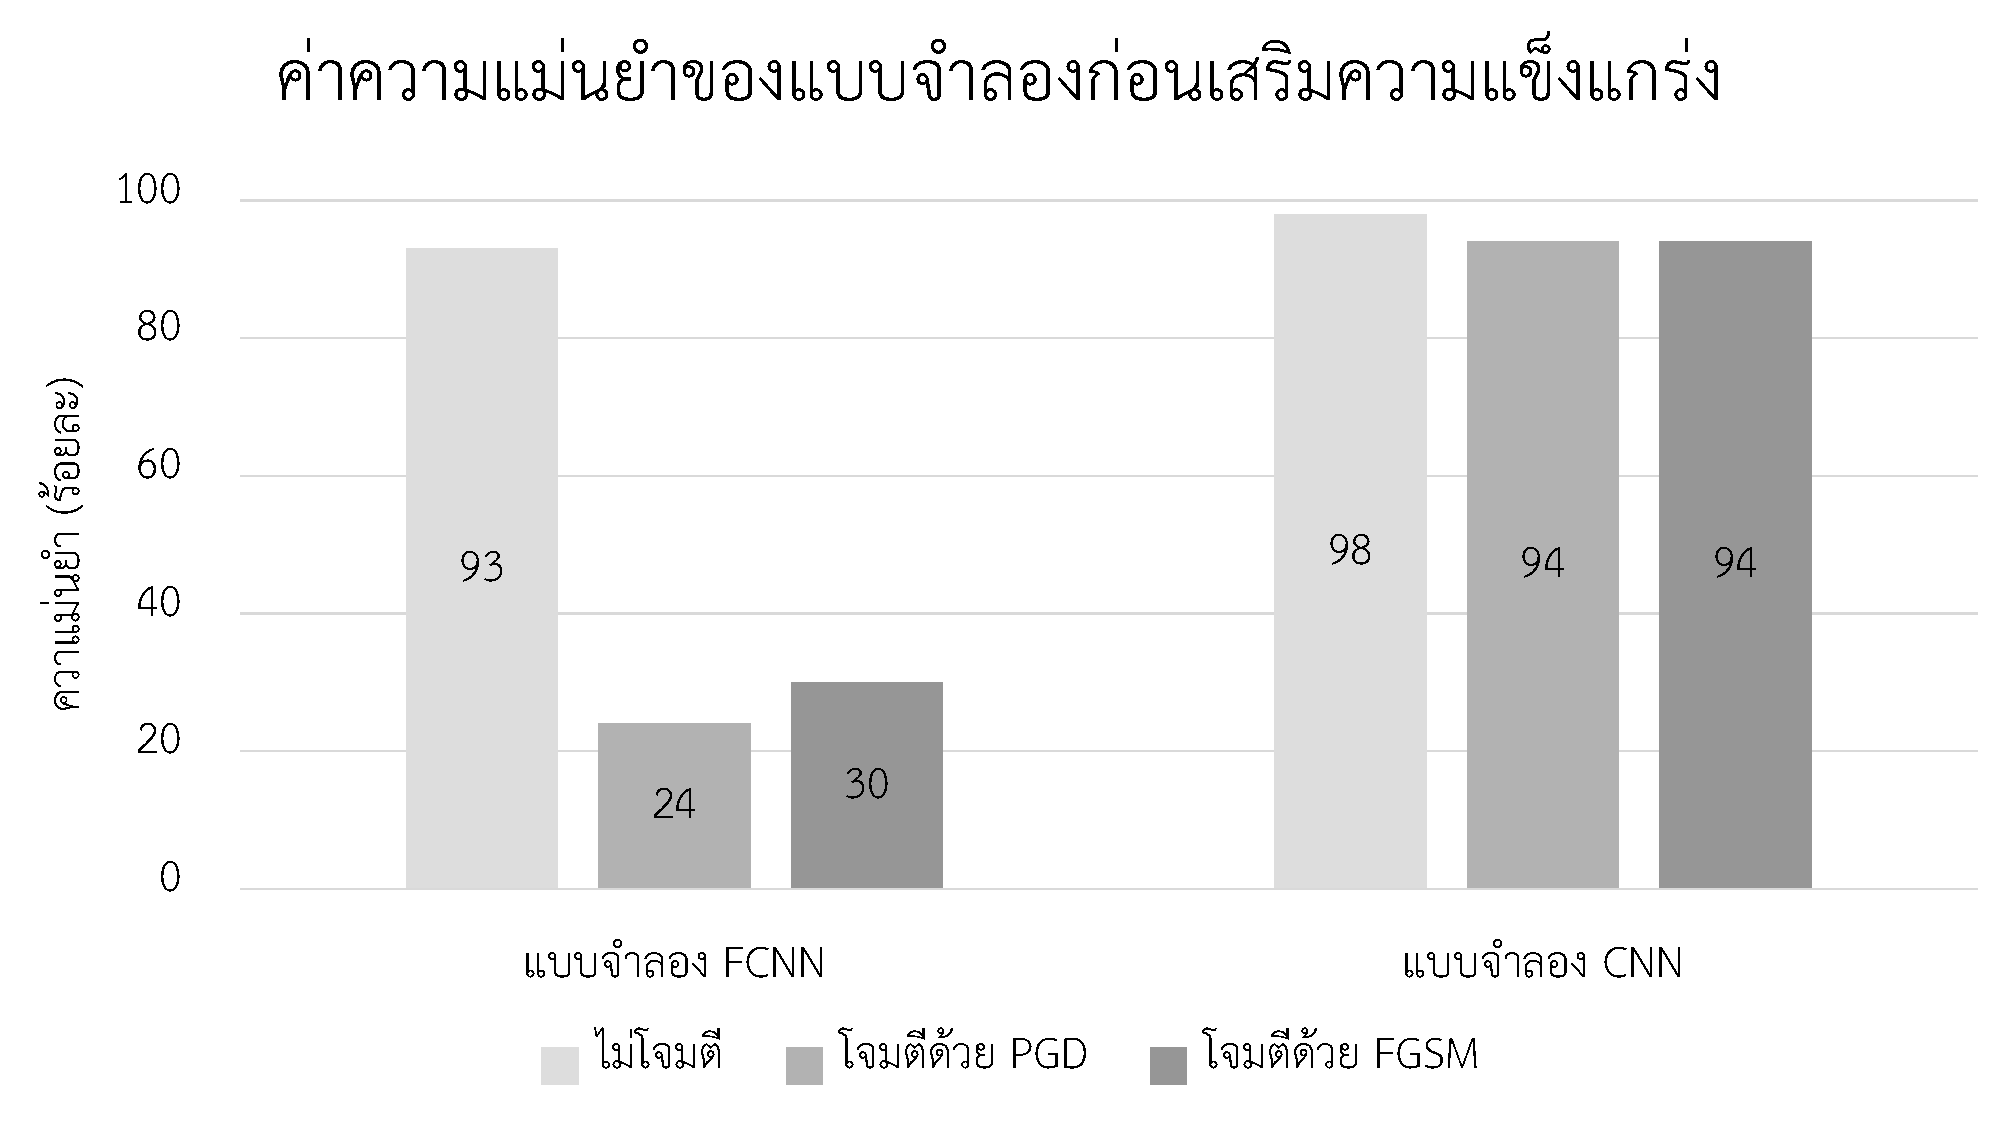
\includegraphics[width=0.8\textwidth]{images/acc-before.pdf}
    \caption{ค่าความแม่นยำของแบบจำลองก่อนเสริมความแข็งแกร่ง}
    \label{acc-before}
\end{figure}

\subsection{การเสริมความแข็งแกร่งแบบจำลองด้วยการฝึกสอนใหม่}

เมื่อวัดผลการโจมตีแบบจำลองได้แล้ว ผู้จัดทำทดลองเสริมความแข็งแกร่งแบบจำลองด้วยวิธีการมาตรฐาน (ขั้นตอนวิธีที่ \ref{retrain}) เทียบกับขั้นตอนวิธีที่โครงงานวิศวกรรมคอมพิวเตอร์นี้เสนอ (ขั้นตอนวิธีที่ \ref{cluster-retrain}) โดยทำการฝึกสอนใหม่จำนวน $e=10$ รอบ ขนาดชุดฝึกสอนเล็กจิ๋วสำหรับชุดข้อมูลต้นฉบับและชุดข้อมูลประสงค์ร้ายเท่ากับ $m=64$ และ $m'=32$ ตามลำดับ น้ำหนักที่ถ่วงสำหรับชุดข้อมูลต้นฉบับและชุดข้อมูลประสงค์ร้ายเท่ากับ $w=1$ และ $w'=2$ ตามลำดับ

\subsection{การวัดประสิทธิภาพการเสริมความแข็งแกร่ง}

เราวัดประสิทธิภาพของการเสริมความแข็งแกร่งโดยอิงจากปัจจัยเวลาที่ใช้ในการฝึกสอนแบบจำลองใหม่ และความแม่นยำของแบบจำลอง รูปที่ \ref{time-used} และ \ref{acc-after} แสดงให้เห็นถึงเวลาที่ใช้ในการฝึกสอนทั้งหมด และความแม่นยำหลังจากการฝึกสอน

\begin{figure}
    \centering
    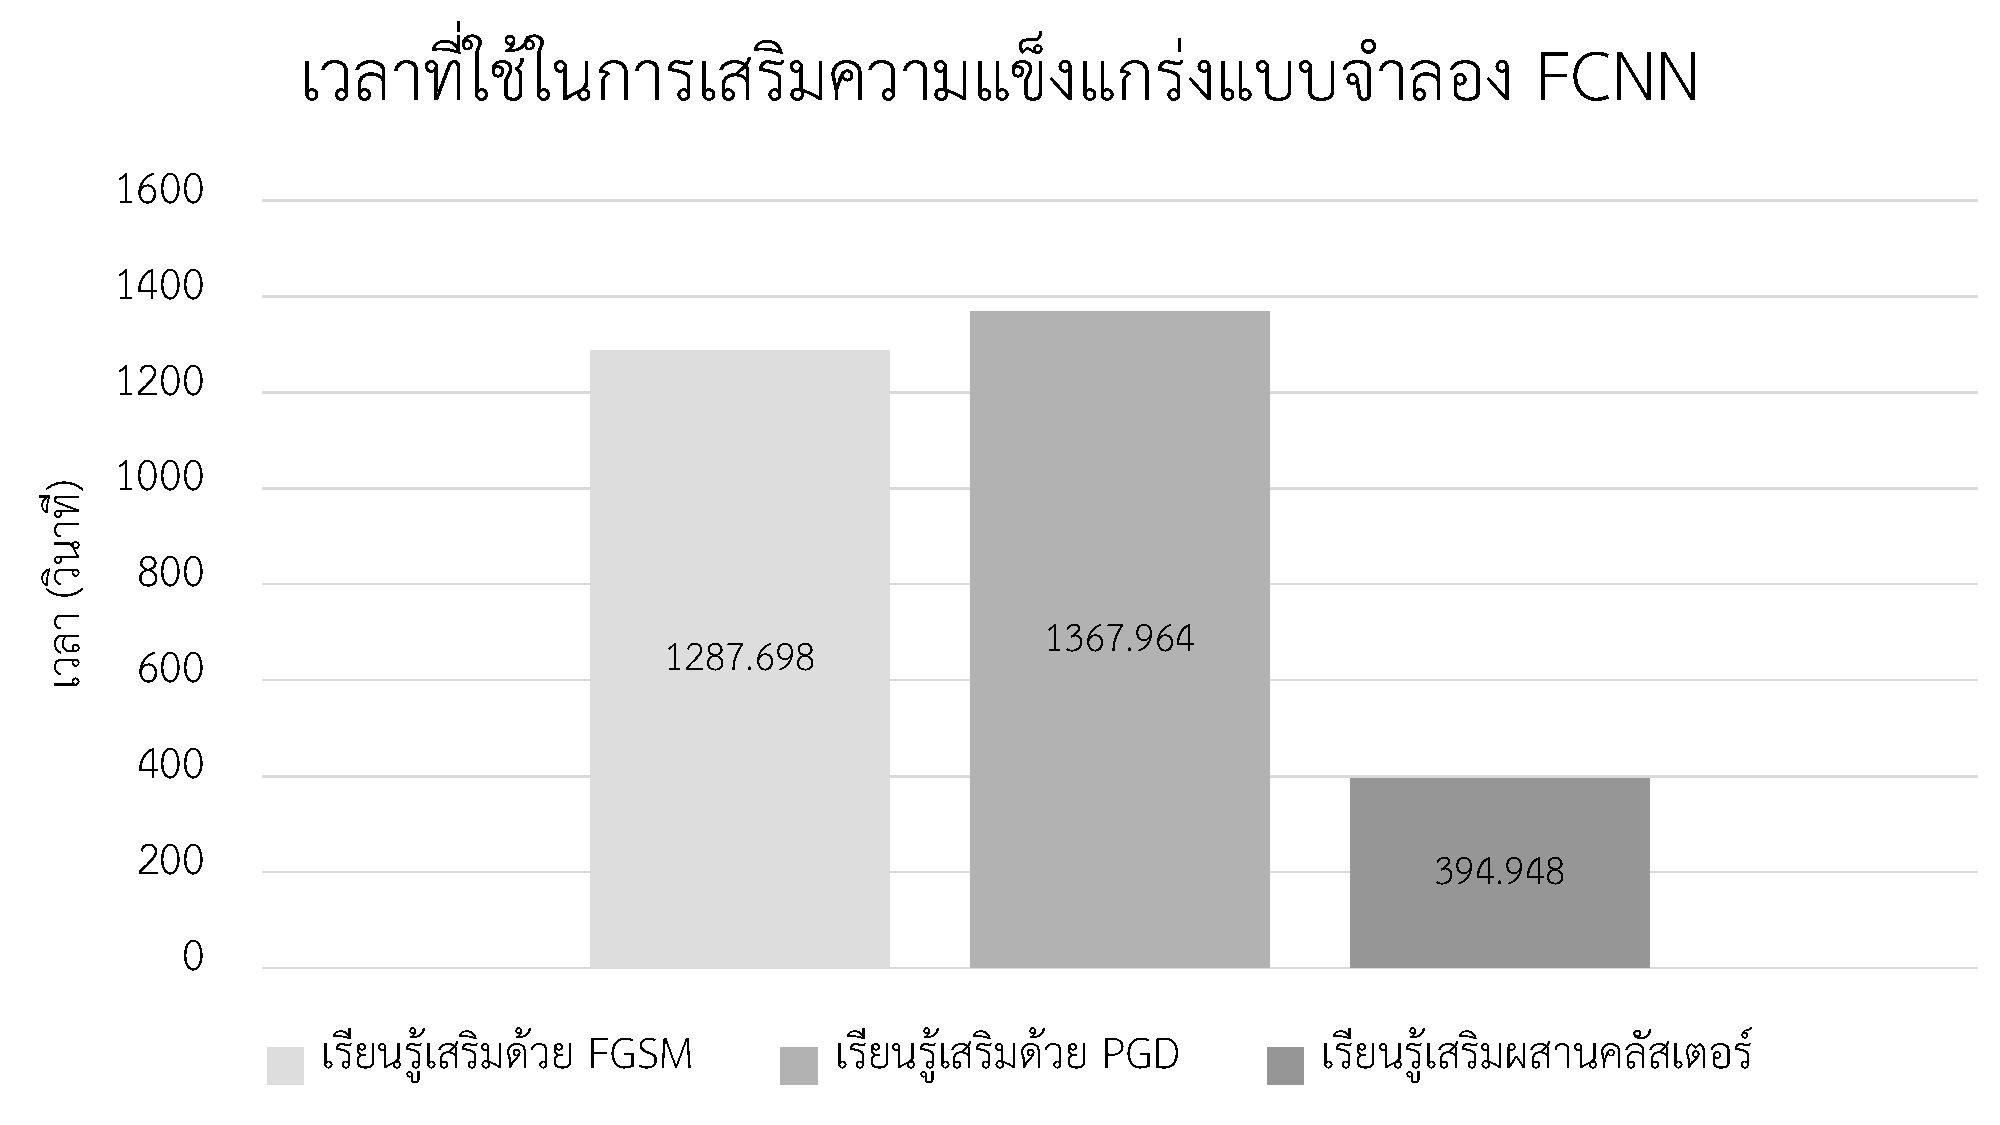
\includegraphics[width=0.8\textwidth]{images/time.pdf}
    \caption{เวลาที่ใช้ในการเสริมความแข็งแกร่งแบบจำลอง}
    \label{time-used}
\end{figure}

\begin{figure}
    \centering
    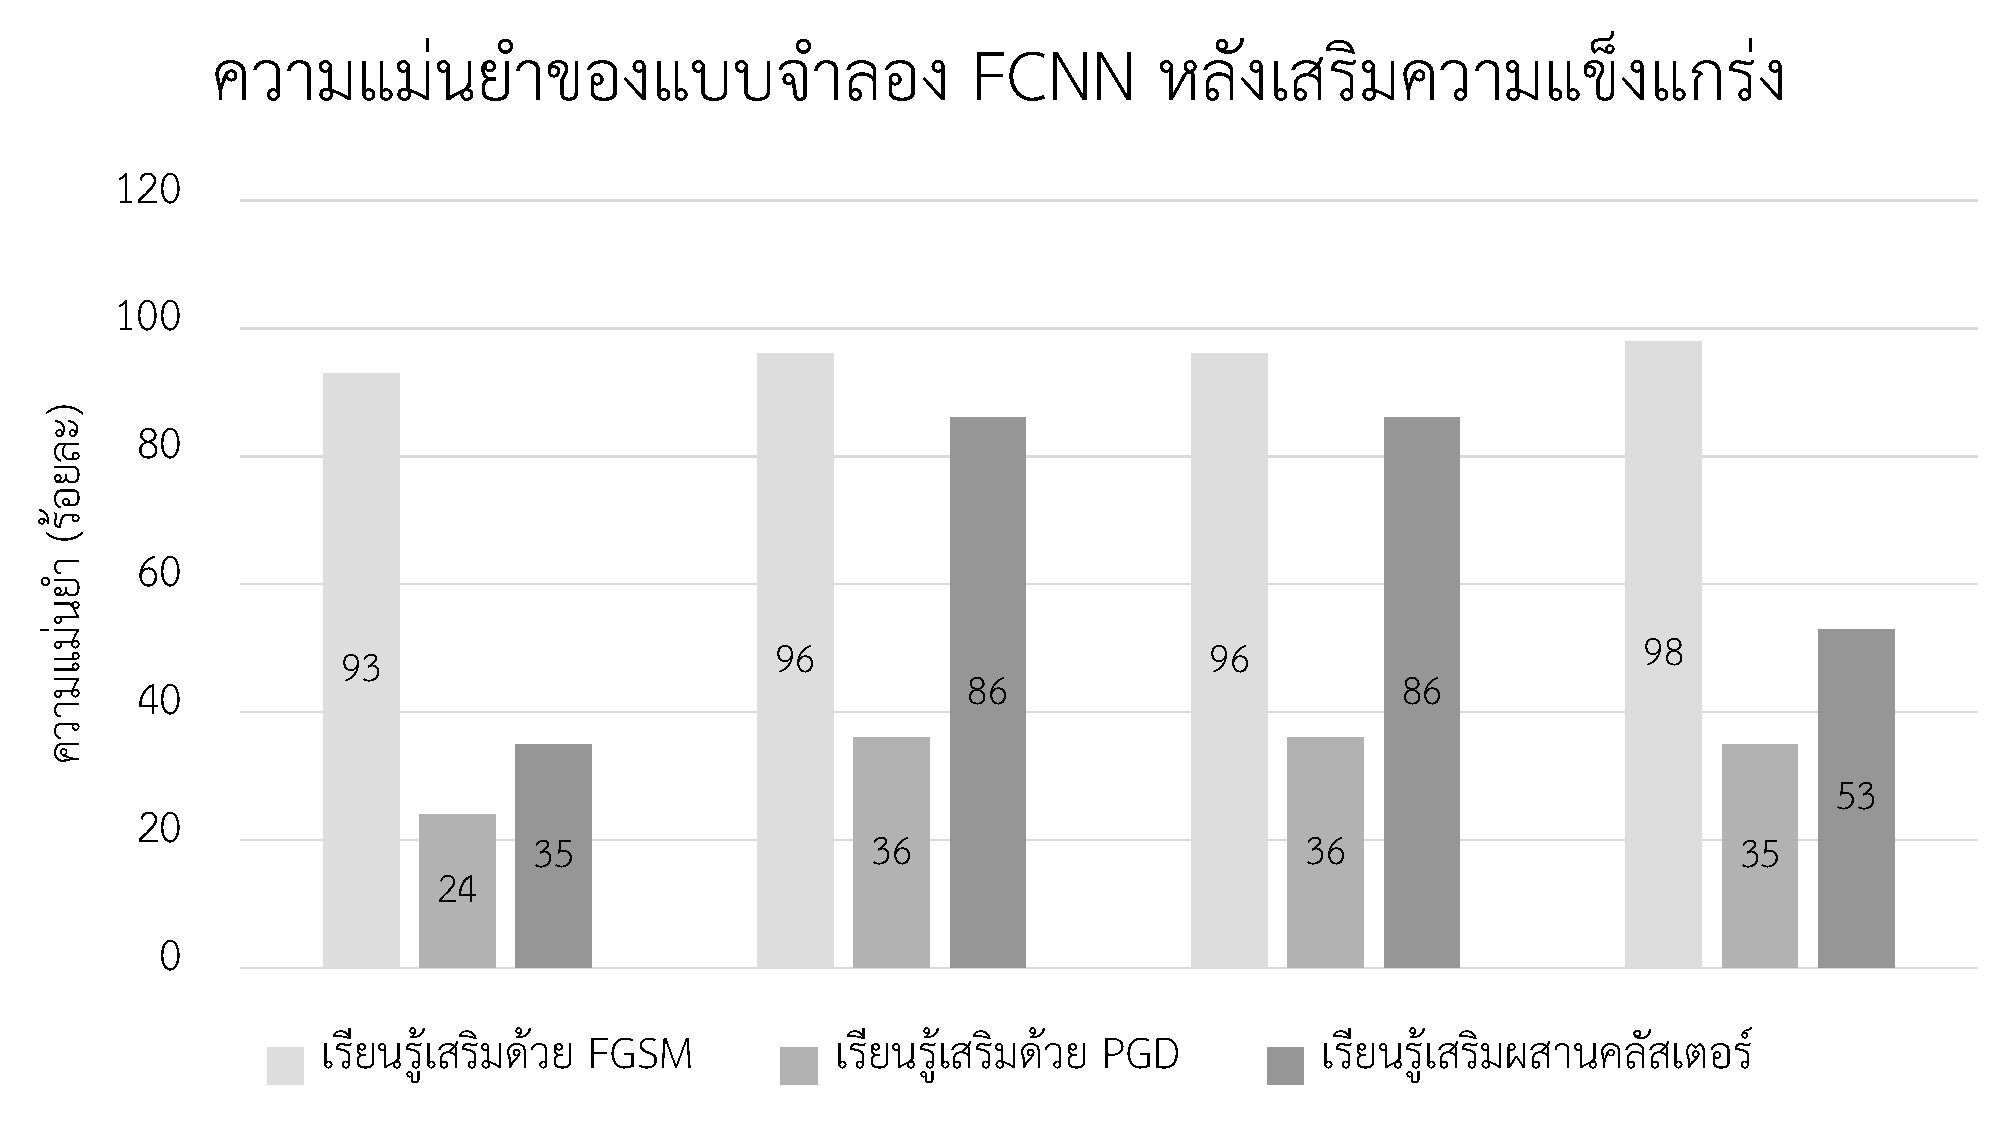
\includegraphics[width=0.8\textwidth]{images/fcnn-acc-after.pdf}
    \caption{ค่าความแม่นยำของแบบจำลอง CNN หลังเสริมความแข็งแกร่ง}
    \label{acc-after}
\end{figure}

\section{การวิเคราะห์ผล}

แม้ว่าขั้นตอนวิธีที่เสนอจะไม่สามารถสร้างให้แบบจำลองทนทานต่อการโจมตีแบบ FGSM ได้ แต่แบบจำลองที่ผ่านการเสริมความแข็งแกร่งนั้นทนทานต่อการโจมตีแบบ PGD มากขึ้นเทียบเท่าวิธีอื่น ในระบะเวลาเสริมความแข็งแกร่งที่น้อยลงประมาณ 3 เท่าตัว